
\setcounter{chapter}{1}
\chapter{Requirements analysis and specification}
\minitoc %insert la minitoc
\graphicspath{{Chapter2/figures/}}

%\DoPToC

%==============================================================================
\pagestyle{fancy}
\fancyhf{}
\fancyhead[R]{\bfseries\rightmark}
\fancyfoot[R]{\thepage}
\renewcommand{\headrulewidth}{0.5pt}
\renewcommand{\footrulewidth}{0pt}
\renewcommand{\chaptermark}[1]{\markboth{\MakeUppercase{\chaptername~\thechapter. #1 }}{}}
\renewcommand{\sectionmark}[1]{\markright{\thechapter.\thesection~ #1}}

\begin{spacing}{1.2}
%==============================================================================
\section*{Introduction}
In this chapter we will begin our project by a study of the existing checkout developers API's on the market, then we will start the requirements analysis to identify the different actors that will interact with our system, as well as the features required in our project.
\section{Study of the existing}
In The world of e-commerce, a lot of payments methods exists.  Most of the methods are credit card related and offer the possibility to pay using the card number and the three digits code.

In our case, Flouci offer payments through QR codes scans. Although the payment steps on the user side are different, the developer API should offer similar functionalities.


Below is a list of world leader online payment API's:
\begin{itemize}
  \item \textbf{Stripe:}

 The Stripe API is organized around REST. The API has predictable resource-oriented URLs, accepts form-encoded request bodies, returns JSON-encoded responses, and uses standard HTTP response codes, authentication, and verbs.

You can use the Stripe API in test mode, which does not affect your live data or interact with the banking networks. The API key you use to authenticate the request determines whether the request is live mode or test mode.

The figure \ref{fig:stripe} shows the code behind stripe integration.
\begin{figure}[!ht]\centering
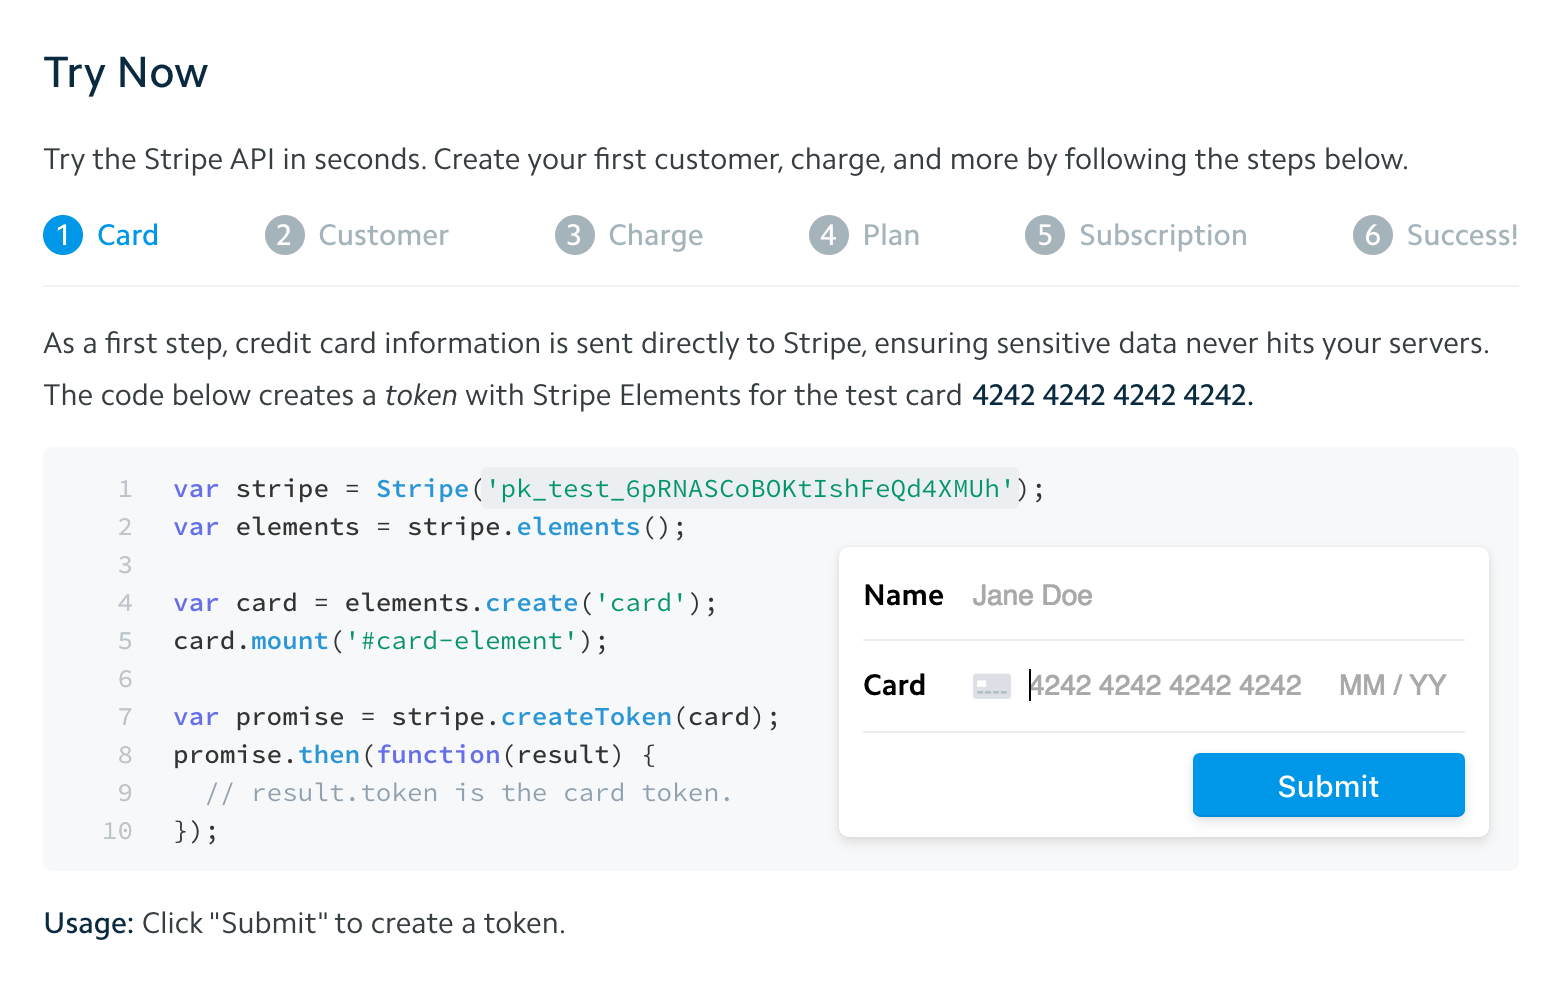
\includegraphics[scale=0.3]{stripe.png}
\caption{Stripe Api}
\label{fig:stripe}
\end{figure}

  \item \textbf{Paypal:}

  The PayPal APIs are HTTP-based RESTful APIs that use OAuth 2.0 for authorization. API request and response bodies are formatted in JSON.
  
The figure \ref{fig:paypal} shows the develeopers API of Paypal.
\begin{figure}[!ht]\centering
\includegraphics[scale=0.3]{PayPal.png}
\caption{PayPal Api}
\label{fig:paypal}
\end{figure}
\newpage
\item \textbf{Twint:}

Twint is the closest implementation to Flouci, it offers payments through QR code scans.

The plugin allows QR code generation on the web page, it also creates a code for each transaction, It serves to confirm payments.
The figure \ref{fig:twint} shows the Twint payment interface.
\begin{figure}[!ht]\centering
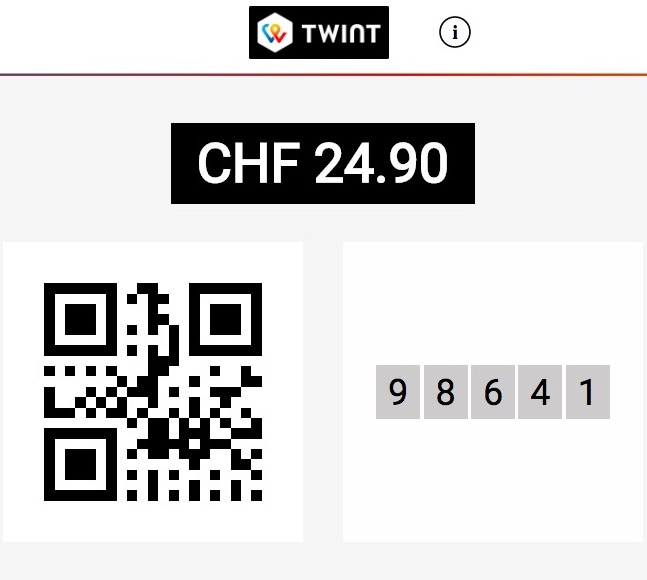
\includegraphics[scale=0.3]{twint.jpg}
\caption{Twint Pop-up}
\label{fig:twint}
\end{figure}
  \end{itemize}
  
  

\section{Requirements specification}
A good in-depth requirements specification is the key to a solid foundation of any project.
The motivation behind this section is to take a global look at the project and be able to understand all the requirements needed to achieve our goals.
\subsection{Actors identification}
Actors are any entity that plays a role in our system. They can be users or systems that interact with our system. We were able to identify the external and internal actors of our platform. 
\newline
Among the internal actors we find:
\begin{itemize}
  \item \textbf{Anonymous Developer:} He can navigate on all the public pages of the site which are
accessible without authentication including the documentation part. Also, he can register a developer account.
  \item \textbf{Registred Developer:} He can manage his account, create and manage app's and integrate them on e-commerce websites.
  \item \textbf{Flouci User:}  He can use the checkout API the pay online merchants.
\end{itemize}
The external actors who are necessary for our platform are:
\begin{itemize}
  \item \textbf{Wallets API:} Is needed to activate any app. The app should be linked to a Flouci wallet.
  \item \textbf{Payments API:} Is needed for online payments.
\end{itemize}
\subsection{Functional requirements}
In this section, we will understand the functional requirements of our project by studying the global use case of our system.
	\newline In the Figure \ref{fig:usecasediagram}, we showcase the \textbf{general use case diagram} and then with the Table \ref{tab:usecasediagram} we explain more in-depth the different use cases.
\begin{figure}[H]\centering
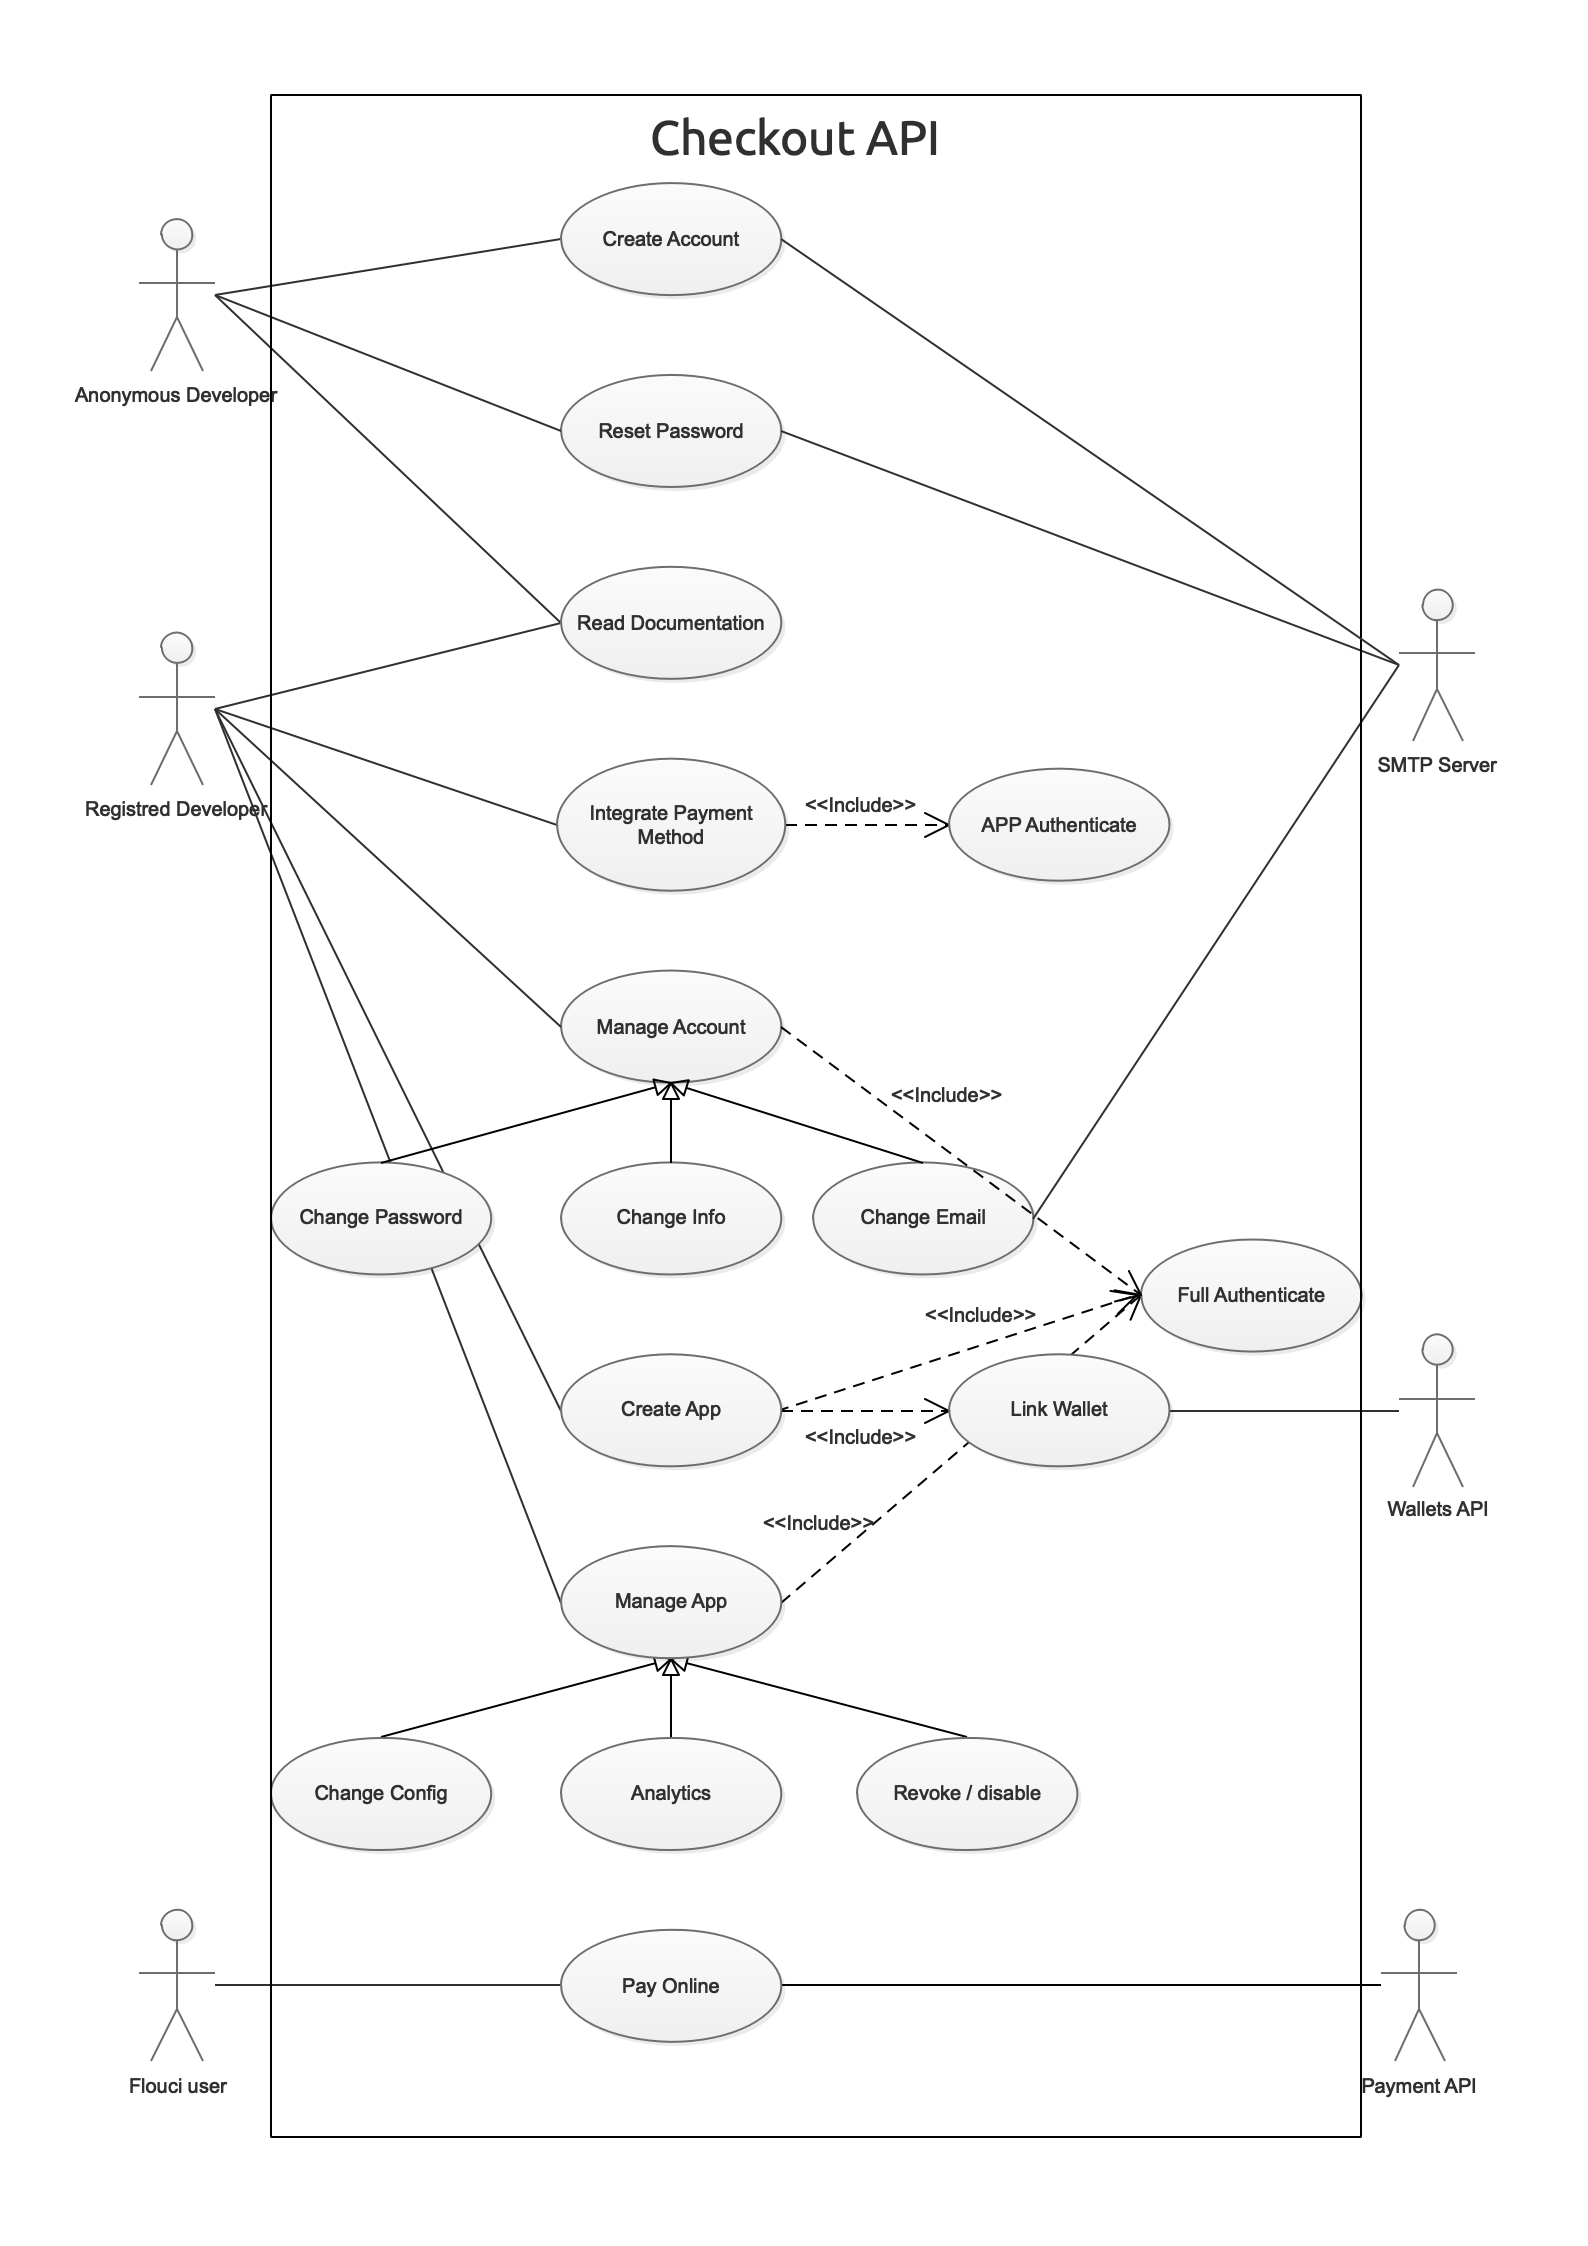
\includegraphics[scale=0.6]{GeneralUseCase.png}
\caption{General Use Case Diagram}
\label{fig:usecasediagram}
\end{figure}

\begin{table}[!h]
	\centering
	\caption{Use case description table}
	\footnotesize
	\begin{tabularx}
	{\linewidth}{|>{\centering{}\vspace*{\fill}}X|>{\centering{}\vspace*{\fill}}X|>{\vspace*{\fill}}X<{\centering{}}|}	
			\hline 
			 \bfseries Internal actor & \bfseries Use case &\bfseries External actor \\
			\hline 
			\multirow{3}{*}{Anonymous Developer}			&	Create Account: Any person with an email account can register for a Flouci developer account. 	&	SMTP Server			\\
			\cline{2-3}
				& Reset Password: In case a registered user forgets his password, he can reset it using his email address. 		&		SMTP Server		\\
				\cline{2-3}
					&	Read Documentation: Any person with access to the developer's platform can access the documentation.	&				\\
			\hline 
			\multirow{5}{*}{Registred Developer}					&	Read Documentation: The developer can access the documentation 	&				\\
			\cline{2-3}
			&	Integrate Payment Method: Any active app could be integrated into a commerce website and the integration only requires the public and private app tokens (App Authentication).	&				\\
			\cline{2-3}
					&	Manage Account:    The developer can change manage his account by changing his password, email or his basic info.	&		SMTP Server	\\
					\cline{2-3}
					&	Create App: An Authenticated developer can create an app and link it to a wallet with OTP verification through the Wallets API.	&			Wallets API	\\
					\cline{2-3}
					&	Manage App:	 An Authenticated  developer can check the analytics of his apps as well as tweak any app settings. &				\\		
					
			\hline 
			Flouci User	& Pay Online : With the pay with Flouci button on e-commerce websites, the Flouci user can quickly pay online merchants.  	&	Payment API	\\
			
			\hline
	\end{tabularx}
	\label{tab:usecasediagram}
\end{table}


\subsection{Non-functional requirements}
\subsubsection{Security}
When it comes to payment solutions security is the number one requirement to keep in mind.
Our solution implements many layers of security including: 
\begin{itemize}
	\item \textbf{HTTPS:} The platform only works on https mode, we use "Kaoun" trusted certificate.
	\item \textbf{JWT Token\cite{JWT}:}  Access to the platform is secured with JWT tokens, managing apps is only possible with this token.
	\item \textbf{Private / Public Tokens for Apps:}  In order to accept Payments Flouci user sign payments attached to the app public key and the developer can only accept them if he has the private key.
	App public keys can be revoked.
\end{itemize}
\subsubsection{Documentation}
An API is only usable with proper documentation, So in order to get developers to implement our solutions, we should have easy and understandable documentation. The documentation is accessible in our platform.\subsubsection{Logging}
Our Solution is using "logstash" to forward logs to our ELK\cite{ELK} stack, different log levels are used and we implemented a lot of metrics and dashboards on our kibana.
The figure below \ref{fig:kibana} shows the logging dashboard of Kibana.
\begin{figure}[H]\centering
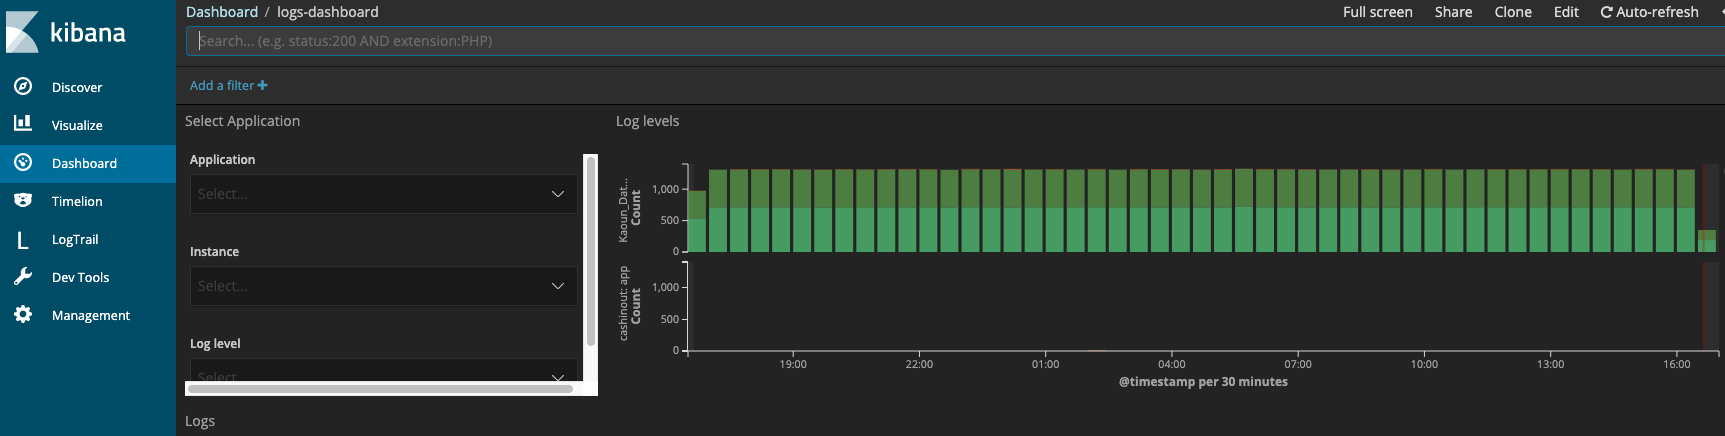
\includegraphics[scale=0.3]{ELK.png}
\caption{Kibana Dashboard}
\label{fig:kibana}
\end{figure}

\subsubsection{Integrability}
Flouci online payment method can be easily integrated into any e-commerce website. It only requires an HTML form in the front end and an API call to accept payments on the backend.

\subsubsection{Extensibility}
Our payment method should allow extensibility and add more payment method other than the QR code scans. 
\subsubsection{Legal}
On the legal side, we should be compliant with the Tunisian laws and only enable appropriate users to accept payments.
This is achieved on the app creation level, at the stage of linking the wallet.
\subsubsection{Privacy}
Flouci users privacy should be considered at the highest levels, payment history and activities should be seen only by the persons with the right permissions.
\subsubsection{Ergonomics}
To guarantee a good control of our project and to simplify the interaction with the final users, we support our analysis of functional needs with mock-ups that model the different interfaces of our final product. These models are made by the "Adobe XD" tool and they are compliant with the overall Kaoun prouducts user experience. \newline Figure \ref{checkoutScreen} represents the checkout pop-up on e-commerce websites.
\newline Figure \ref{developersPlatform} represents the Developers API platform.

\begin{figure}[H]\centering
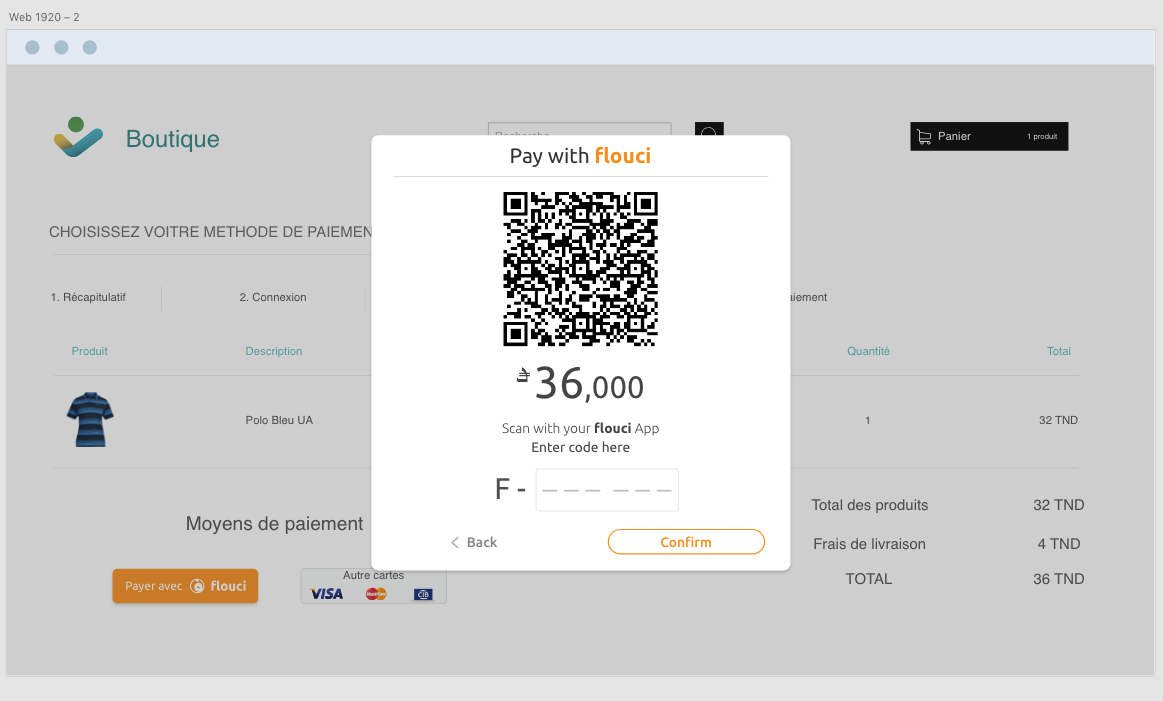
\includegraphics[scale=0.3]{Checkout_screen}
\caption{Checkout pop-up mock-up}
\label{checkoutScreen}
\end{figure}

\begin{figure}[H]\centering
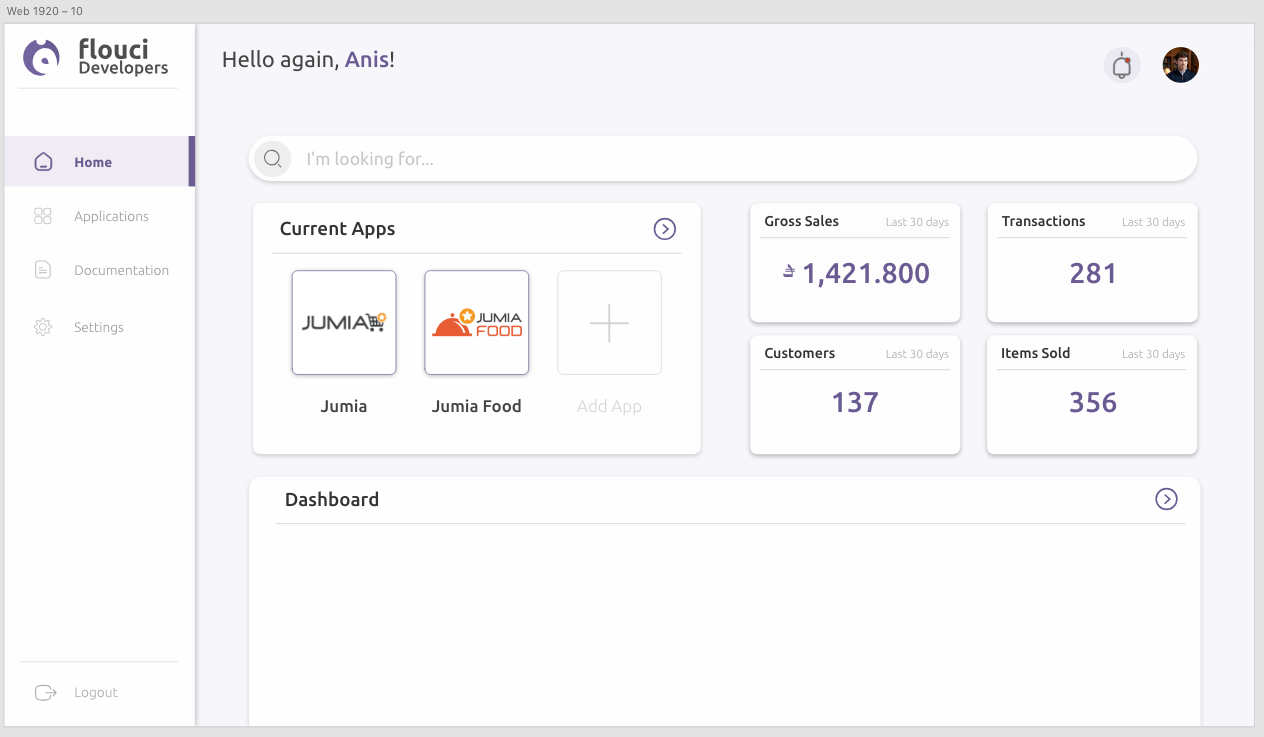
\includegraphics[scale=0.4]{web_screen}
\caption{Developers platform mock-up}
\label{developersPlatform}
\end{figure}

\section*{Conclusion}
In this chapter, we took the time to think about different aspects of our project, we went through detailed analysis in order to comprehend the project boundaries. After this we can launch our project development cycles which what we will be the topic of our next chapter.
%==============================================================================
\end{spacing}
